\documentclass[]{article}

%%%%%%%%%%%%%%%%%%%
% Packages/Macros %
%%%%%%%%%%%%%%%%%%%
\usepackage{amssymb,latexsym,amsmath,graphicx}     % Standard packages
\usepackage[utf8]{inputenc} % Implementere Unicode
\usepackage{multirow}
\renewcommand{\tablename}{Tabel}

%%%%%%%%%%%
% Margins %
%%%%%%%%%%%
\addtolength{\textwidth}{1.0in}
\addtolength{\textheight}{1.00in}
\addtolength{\evensidemargin}{-0.75in}
\addtolength{\oddsidemargin}{-0.75in}
\addtolength{\topmargin}{-.50in}


%%%%%%%%%%%%%%%%%%%%%%%%%%%%%%
% Theorem/Proof Environments %
%%%%%%%%%%%%%%%%%%%%%%%%%%%%%%
\newtheorem{theorem}{Theorem}
\newenvironment{proof}{{\bf Bevis:}}{$\hfill \Box$ \vspace{10pt}}

%%%%%%%%%%%%
% Document %
%%%%%%%%%%%%
\begin{document}

\title{Kopier denne \LaTeX ~fil!}
\author{Arinbjörn, Benjamin \& Mathias}
\date{12. oktober, 2015}
\maketitle
\tableofcontents

\begin{abstract}

Det her dokument indeholder en masse af de ting, som man normalt vil få brug for. Lav en ny \LaTeX fil og se om du kan få det til at se ud præcist som dette! Brug det udleverede cheat sheet, for der vil uden tvivl være nogle kommandoer du ikke kan huske udenad. Endvidere kan $detexify.kirelabs.org$ benyttes til at finde koden for symboler man ikke kan huske. En skabelon til dette dokument kan findes på $rotendahl.dk/skabelon.tex$. Skabeloner til andre dokumenter du kunne finde på at lave, eksempelvis din SRP, kan findes på $latextemplates.com$.


$$
\left(
\begin{array}[c]
    n \\
    i
\end{array}
\right)
$$


\end{abstract}
\newpage

\section{Lister}
\begin{enumerate}
\item {\bf Første punkt (Fed skrift)}
\item {\em Andet punkt (I kursiv)}
\item {\Large Tredje punkt (Stor skrift)}
    \begin{enumerate}
        \item {\small Første underpunkt (Lille skrift)}
        \item {\tiny Andet underpunkt (Endnu mindre skrift)}
        \item {\Huge Tredje underpunkt (Kæmpe skrift)}
    \end{enumerate}
\item[$\bullet$] {\sf Bullet Point (Sans Serif)}
\item[$\circ$] {\sc Circle Point (Small Caps)}
\end{enumerate}


\section{Ligninger}
\subsection{Binomial Theorem}

\begin{Theorem}[Binomial Theorem]
For ethvert ikke-negativt heltal $n$, har vi at
\[
	(1+x)^n = \sum_{i=0}^n {n \choose i} x^i
\]
\end{Theorem}

\subsection{Taylor Serier}
Taylor\footnote{Der er her ikke tale om Taylor Swift. Læs mere på $https://en.wikipedia.org/wiki/Taylor\_series$}-udvidelsen for funktionen $e^x$ er givet ved
\[
	e^x = 1 + x + \frac{x^2}{2} + \frac{x^3}{6} + \cdots = \sum_{n\geq 0} \frac{x^n}{n!}
\]

\section{Tabeller}
Lad os lave nogle tabeller!

\begin{center}
	\noindent
	\begin{tabular}{l||c|r}
		venstrestillet & midterstillet & højrestillet \\ \hline
		1 & 3.14159 & 5 \\
		2.4678 & 3 &  1234 \\ \hline \hline
		3.4678 & 6.14159 & 1239
	\end{tabular}
\end{center}


Mon man kan samle rækkerne i en tabel?

\begin{center}
	\noindent
	\begin{tabular}{|c|c|c|c| }
		\hline
		 & Forsøg 1 & Forsøg 2 \\
		\hline
		\multirow{3}{4em}{Antal ramte} & 4 & 3 \\
									   & 5 & 5 \\
									   & 2 & 4 \\
		\hline
	\end{tabular}
\end{center}
\newpage

Hvad med kolonnerne?
\begin{table}[h]
	\begin{center}
		\begin{tabular}{ |p{3cm}|p{3cm}|p{3cm}|  }
		\hline
		\multicolumn{3}{|c|}{Country List} \\
		\hline
		Land/område& ISO ALPHA 2 &ISO ALPHA 3 \\
		\hline
		Afghanistan & AF & AFG \\
		Aland Islands & AX   & ALA \\
		Albania &AL & ALB \\
		Algeria    &DZ & DZA \\
		American Samoa & AS & ASM \\
		Andorra & AD & AND   \\
		Angola & AO & AGO \\
		\hline
		\end{tabular}
		\caption{Det kunne man sørme godt!}
	\end{center}
\end{table}

\begin{figure}[ht!]
	\centering
	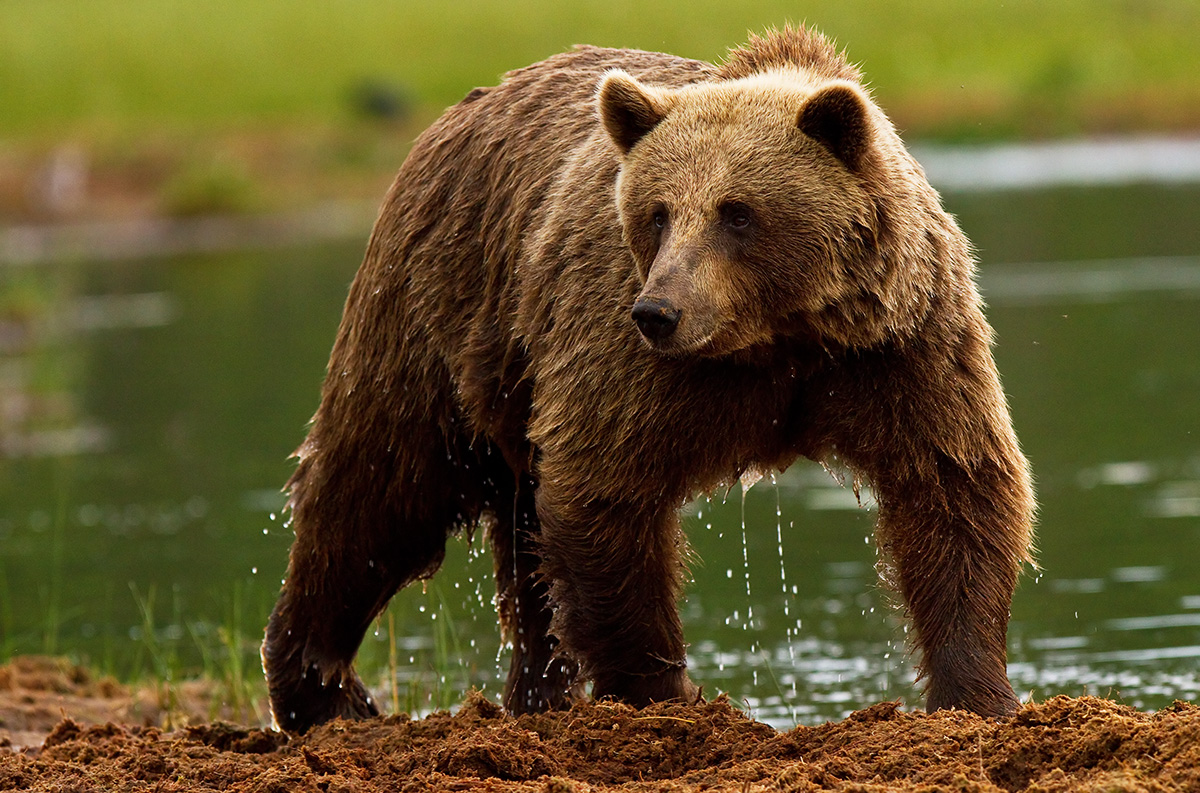
\includegraphics[width=65mm]{bear.jpg}
	\caption{Hjælp! En bjørn angriber min pdf! \label{overflow}}
\end{figure}

\section{Andre Matematiske Udtryk}
Her er lidt ekstra matematiske udtryk

\subsection{Diverse}
\begin{flalign*}
	a &= \left(a + b \right) \left[1 - \frac{b}{a + b} \right] \,, \\
	\sqrt{|xy|} &\leq \left| \frac{x + y}{2} \right|\,, \\
	\int_a^b u \frac{d^2 v}{dx^2}dx &= u \frac{dv}{dx}
	- \int_a^b \frac{du}{dx} \frac{dv}{dx} dx\,, \\
	|x|&=\begin{cases}
		x, & \text{if }x\geq 0\,,  \\
		-x, & \text{if }x< 0\,.
	\end{cases}
\end{flalign*}

\subsection{Matricer}
\[
	\begin{bmatrix}
		1 & x & 0 \\
		0 & 1 & -1
	\end{bmatrix}
	\begin{bmatrix}
		1  \\
		y  \\
		1
	\end{bmatrix}
	=
	\begin{bmatrix}
		1+xy  \\
		y-1
	\end{bmatrix}\,,
\]
\[
	\begin{matrix}
		-2 & 1 & 0 & 0 & \cdots & 0  \\
		1 & -2 & 1 & 0 & \cdots & 0  \\
		0 & 1 & -2 & 1 & \cdots & 0  \\
		0 & 0 & 1 & -2 & \ddots & \vdots \\
		\vdots & \vdots & \vdots & \ddots & \ddots & 1  \\
		0 & 0 & 0 & \cdots & 1 & -2
	\end{matrix}
\]

\subsection{Funktioner}
\noindent
\[
	\exp(i \theta) = \cos \theta + i \sin \theta\,, \quad
	\sinh(\log x) = \frac{1}{2} \left(x - \frac{1}{x} \right)
\]

Og så lidt mere komplicerede funktioner
\begin{flalign*}
	\lim_{q \to \infty} \|f(x)\|_q &= \max_{x}|f(x)|, \\
	e^x &= \sum_{n = 0}^\infty \frac{x^n}{n!} \quad
	\text{where } n! = \prod_{i = 1}^n i\,,  \\
	\overline{U_\alpha} &= \bigcap_\alpha U_\alpha\,.
\end{flalign*}

Når man skriver inline matematik sørger \LaTeX selv for at det vertikale mellemrum passer som i følgende:
$1/(1 - x) = \sum_{n = 0}^\infty x^n$.

\subsection{Mængder}
\begin{theorem}
	For enhver mængde $A$, $B$ og $C$, har vi at
	\[
		(A \cup B) - (C-A) = A \cup (B-C)
	\]
\end{theorem}

\begin{proof}
	\begin{flalign*}
		(A \cup B) - (C - A) &= (A\cup B) \cap (C-A)^c \\
		&= (A \cup B) \cap (C \cap A^c)^c \\
		&= (A \cup B) \cap (C^c \cup A) \\
		&= A \cup (B\cap C^c) \\
		&= A \cup (B-C)
	\end{flalign*}
\end{proof}

\end{document}
